\subsection{Moon Survival Prototype}


% objective of game (build base, need oxygen, survive, sandbox)
Moon Survival is a sandbox game based on moon.
The player is man surviving on the moon.
The objective is to survive.
The man needs air to survive, and since their is no air on moon, he must generate air by building a base and adding air generators inside.
The air has basic physics where it will diffuse from a high concentration to an adjacent low concentration.

The style of game is creative open-world, where the player can build whatever he wants, and can experiment with air physics.

The player can build 2 items: 
\begin{description}
\item[air generator] makes air and releases it into its immediate surroundings. 
\item[wall] solid block that blocks the player walking through it as well as air passing through it.
\end{description}

% air physics (diffusion, dissapears at low quantities)
The air physics are highly simplified, to mimic the movement of air without the complexities of the calculations.
Figure \ref{fig:SpaceBaseAirDiffusion} gives an example of air diffusion of 1 iteration. The top diagram in the figure is before the iteration, and the bottom diagram is after the diffusion iteration.
As shown, their air diffuses from a high concentration to low concentration.
The diffusion equation uses the following terms:
\begin{description}
\item[c] function from block to air concentration at that block
\item[t] diffusion rate, constant between 0 and 1 representing transfer rate, 0 is no transfer, 1 is transfer until equilibrium between blocks
\end{description}

For 2 adjacent blocks, b1 and b2, the volume of air that diffuses from b1 to b2 is:
$$ transfer = \frac{c(b1) - c(b2)}{2} * t $$

A problem with the over simplification of the air diffusion, is that this amount of air transferred from the centre block in Figure \ref{fig:SpaceBaseAirDiffusion} is less for each consecutive neighbour, i.e. the first neighbour gets more air than the second neighbour, and the second neighbour gets more air then third neighbour etc.

\begin{marginfigure}
	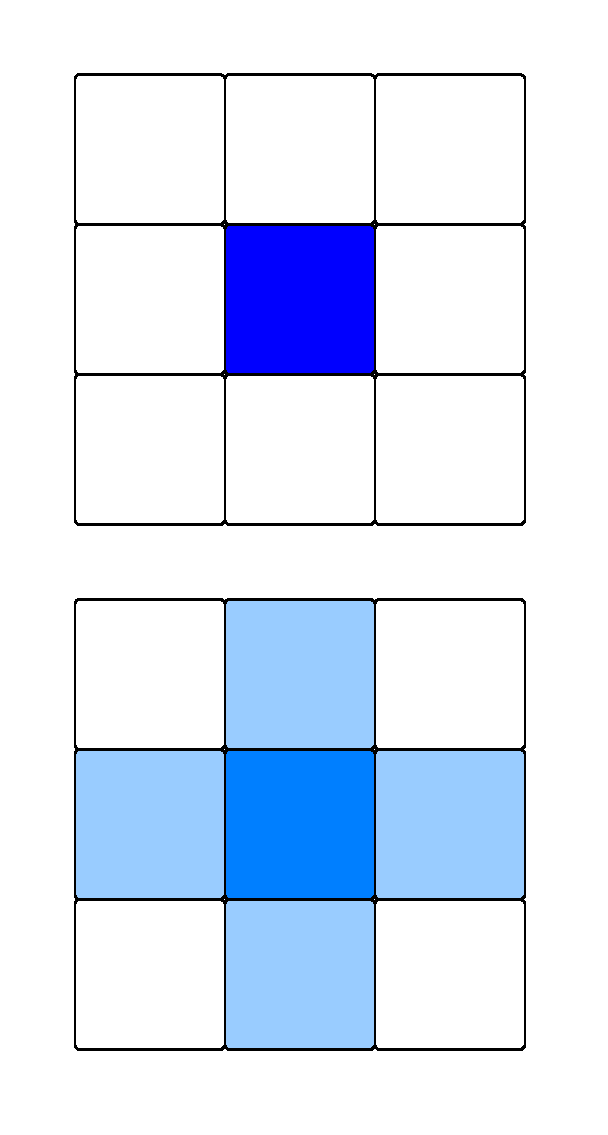
\includegraphics{res/space_base_prototype/MoonSurvivalAirDiffusion.pdf}
	\caption{
	3x3 area, where colour intensity represents volume of air. The higher the colour intensity the more air.
	The top diagram shows the centre square has a high volume of air, and its surrounding squares have no air.
	In the bottom diagram, the air in the centre square has now diffused to its neighbours. Diagonal neighbours are included in this,
	only the square immediately North, East, South, and West of the block are considered neighbours.
	}
	\label{fig:SpaceBaseAirDiffusion}
\end{marginfigure}


% controls (how to move about, collisions)
The player has control of the mans movements as well as what item to place/remove.
The player's movements controls are:
\begin{description}
\item [north] W
\item [east] D
\item [south] s
\item [west] a
\end{description}
Figure \ref{fig:SpaceBaseControls} shows movement controls.
if an obstacle is blocking the way, the player will no move.
A limitation of the movement system is that holding down a key does cause the player to continue to move in that direction, instead the key must be repeatedly tapped to have this effect. This is no limitation, but can be annoying for the player.

The player also has 1 item equipped at any one item, and can switch between the items with the TAB key. The currently selected item is displayed in the command bar (discussed later).

To place an item, press the SPACE key. the item will be placed directly in front of player. 
If the item is already in front of the player and the player presses the SPACE key, the item will be removed.
For example, if the player is standing in front of a wall and facing it, the wall item is selected, and the player hits the SPACE key, that wall will be removed.

\begin{marginfigure}
	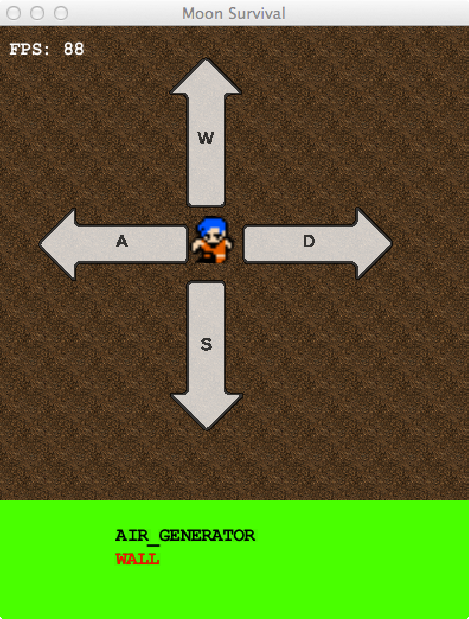
\includegraphics{res/space_base_prototype/MoonSurvivalControls.pdf}
	\caption{MoonSurvivalControls.pdfPlayers controls highlighted}
	\label{fig:SpaceBaseControls}
\end{marginfigure}



% GUI description (what each thing on screen is)



% conclusion (what aspects liked, what aspects were missing, etc)


% missing from the game
The prototype was still in early development stages hence the capabilities of the player is somewhat limited.


This prototype was about building bases on the moon.
The player has control over a man who is able to build the base on the moon.
He has no space suit, so he needs air to breath.

% \begin{marginfigure}[-30em]
\begin{marginfigure}
	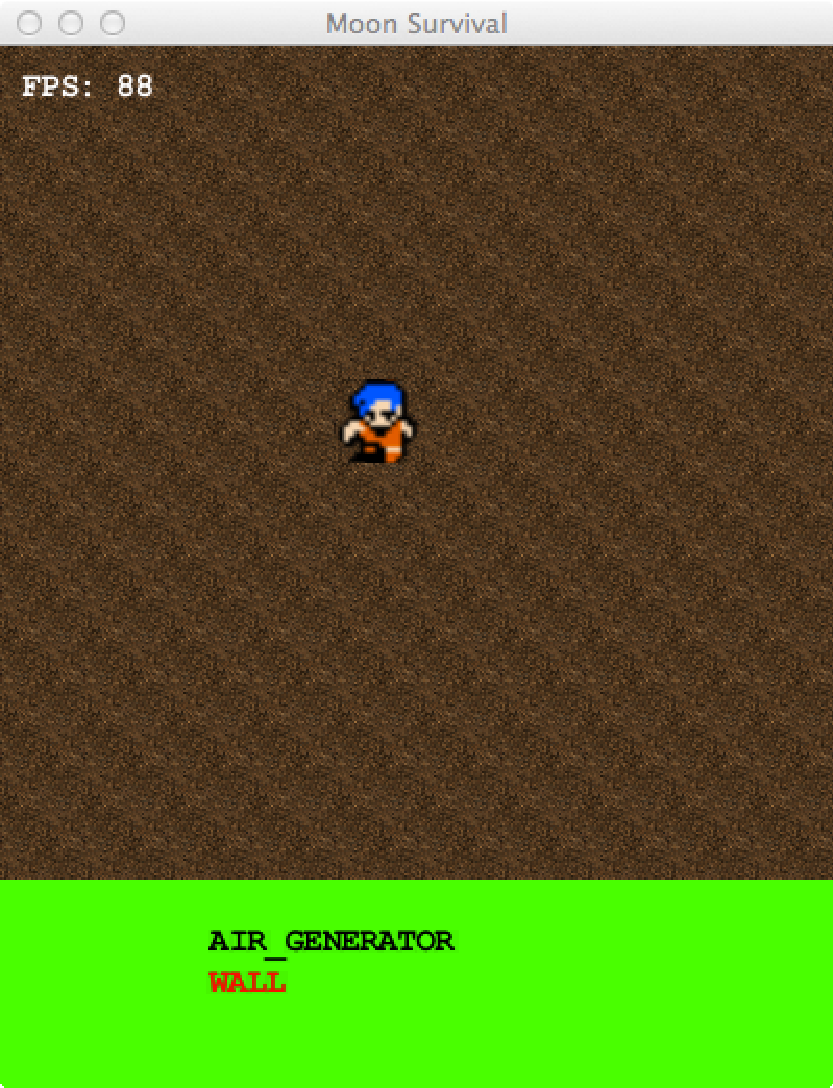
\includegraphics{res/space_base_prototype/no_base.pdf}
	\caption{
	player on moon with no base
	}
	\label{fig:SpaceBaseNoRoom}
\end{marginfigure}

\begin{marginfigure}
	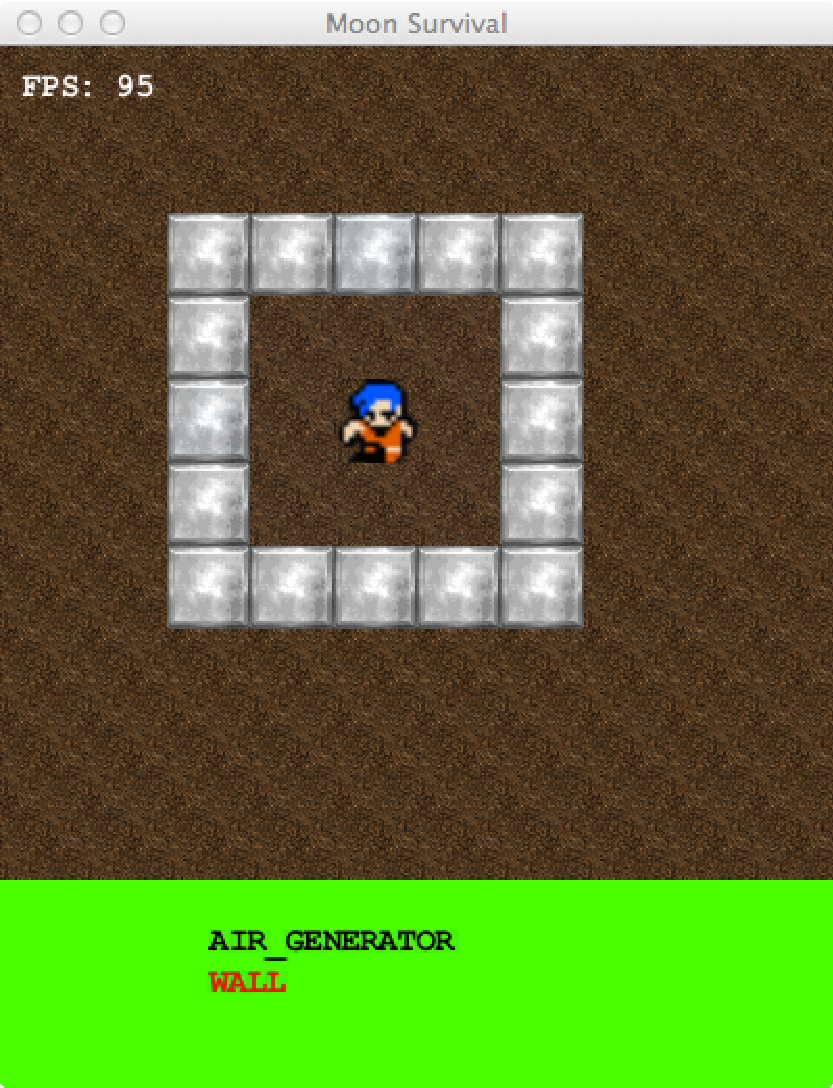
\includegraphics{res/space_base_prototype/empty_room.pdf}
	\caption{
	walled off room with 5x5 interior	}
	\label{fig:SpaceBaseWithRoom}
\end{marginfigure}

\begin{marginfigure}
	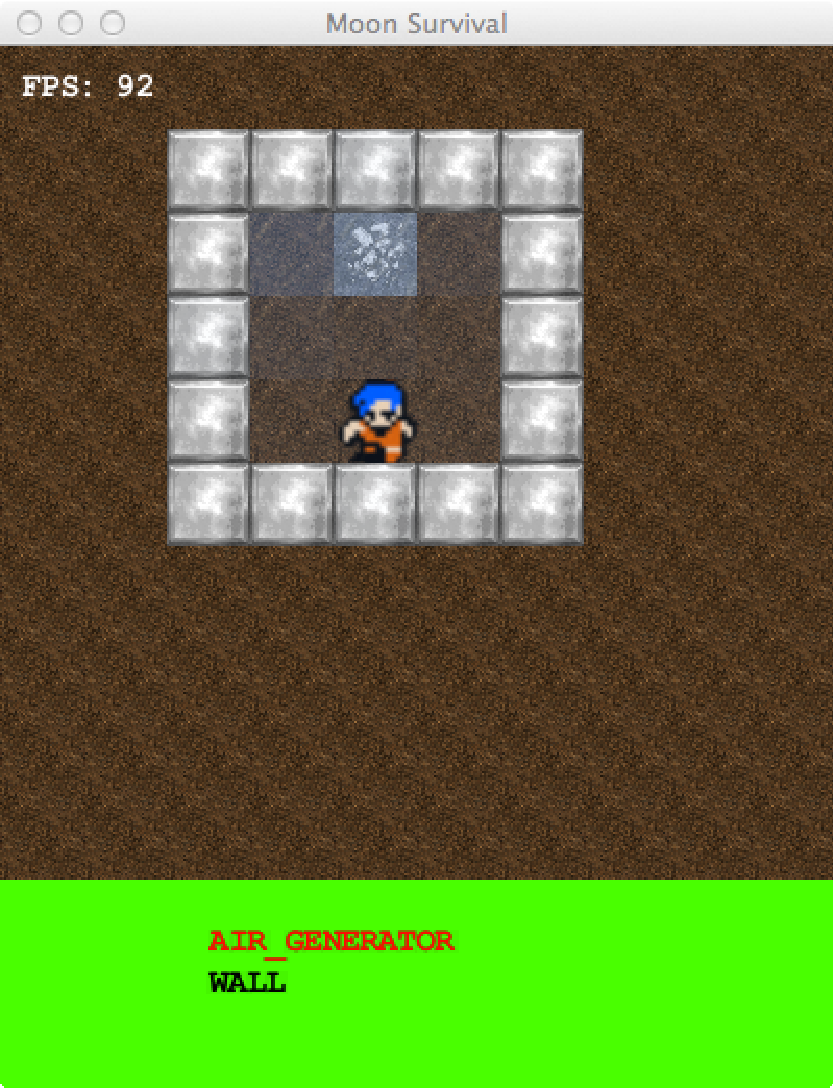
\includegraphics{res/space_base_prototype/room_with_air_generator.pdf}
	\caption{
	walled off room with 5x5 interior and air generator	}
	\label{fig:SpaceBaseWithAirGenerator}
\end{marginfigure}

\begin{marginfigure}
	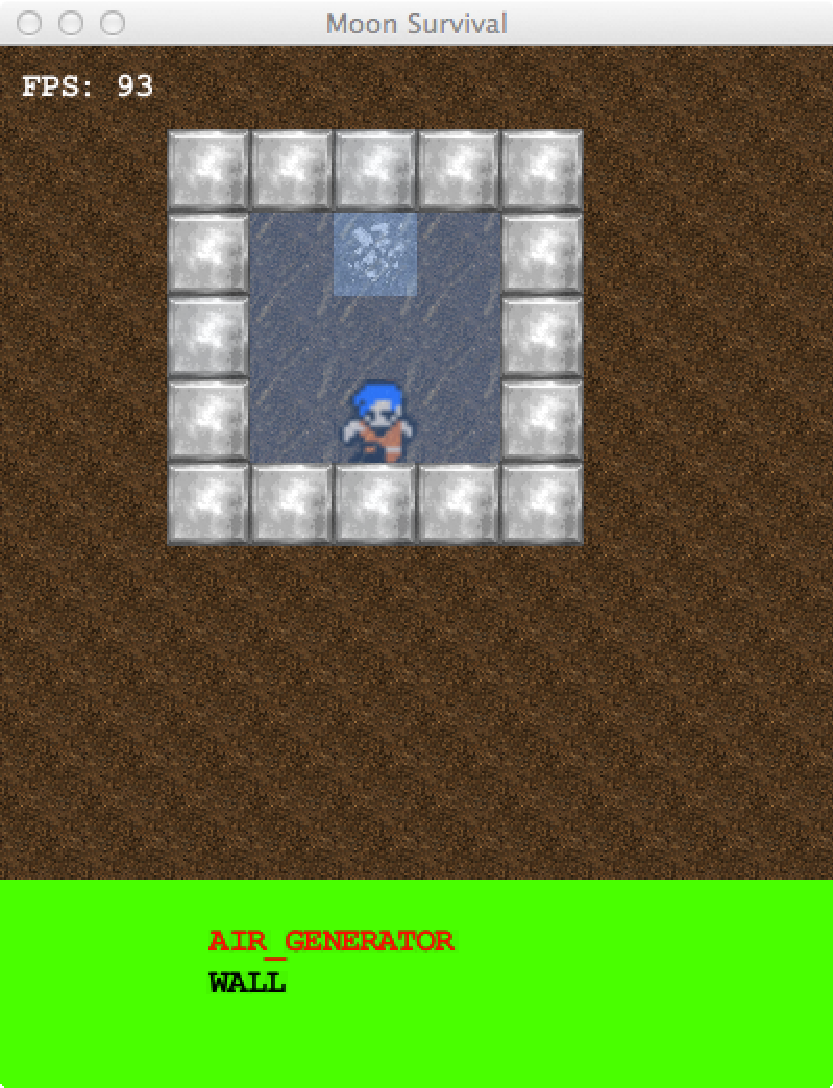
\includegraphics{res/space_base_prototype/room_with_air.pdf}
	\caption{
	walled off room with 5x5 interior and air	
	}
	\label{fig:SpaceBaseWithAir}
\end{marginfigure}



In Figure \ref{fig:spaceBaseNoRoom} the player is in a new game with no air and no base.


The first priority is to build a wall around an area so no air can get out.
This is done by placing wall blocks in front of the player.



In Figure \ref{fig:SpaceBaseWithRoom} the Player has now walled of a room.
The next step to place an air generator within the room as shown in Figure \ref. 
This will start generating air. The air will continue to spread until the entire room is filled. 


% game concept
% - building base on moon
% - air
